\section{Laplace-Transformatio }{135}

Die Laplace-Transformation kann als analytische Fortsetzung der Fourier-Transformation aufgefasst werden. \\
Die Frequenz ist nun komplex $\cbl{(s = \sigma + \jimg \omega)}$ anstelle $\jimg \omega$. Dank dem Dämpfungsfaktor $\sigma$ kann die
Konvergenz von Signalen erzwungen werden.


\subsection{Berechnung der Laplace-Transformation}{135}
\label{Berechnung der Laplace-Transformation}

Komplexe Frequenz: $s = \sigma + \jimg \omega $

$$ \boxed{\text{Laplacetransformation: } F(s) = \int\limits_{0_-}^{\infty} f(t) \, e^{-st} \, \diff t  } $$
$$ \boxed{ \text{Rücktransformation: } f(t) = \frac{1}{2 \pi \jimg} \int\limits_{c - \jimg \infty}^{c+ \jimg \infty} F(s) \, e^{st} \, \diff s  } $$

\textrightarrow\ Für die Rücktransformation werden meistens Tabellen verwendet!


\subsection{Eigenschaften der Laplace-Transformation}{136-138}

\subsubsection{Linearität}

\vspace{-0.2cm}
$$ \boxed{ \alpha \cdot f(t) + \beta \cdot g(t) \, \laplace \, \alpha \cdot F(s) + \beta \cdot G(s)  \quad (\alpha, \, \beta \in \mathbb{C}) } $$


\subsubsection{Ähnlichkeit (Streckung)}

\vspace{-0.2cm}
$$ \boxed{ f(\alpha \, t) \, \laplace \, \frac{1}{| \alpha |} F \Big(\frac{s}{\alpha} \Big) \quad ( 0 < \alpha \in \mathbb{R}) } $$


\subsubsection{Faltung im Zeitbereich (Multiplikation im Frequenzbereich)}

\vspace{-0.2cm}
$$ \boxed{ f(t) * g(t) = \int\limits_{-\infty}^{\infty} f(\tau) \, g(t - \tau) \, \diff \tau 
    = \int\limits_{0}^{t} f(\tau) \, g(t - \tau) \, \diff \tau  \, \laplace \, F(s) \cdot G(s) } $$


\subsubsection{Faltung im Frequenzbereich (Multiplikation im Zeitbereich)}

\vspace{-0.2cm}
$$ \boxed{ f(t) \cdot g(t) \, \laplace \, \frac{1}{2 \pi \jimg} \int\limits_{c- \jimg \infty}^{c + \jimg \infty} F(\xi) * G(s - \xi) \, \diff \xi } $$


\subsubsection{Ableitung(en) im Zeitbereich}

\renewcommand{\arraystretch}{1.5}
\begin{tabular}{r c l}
    $\frac{\diff f(t)}{\diff t}$        & $ \laplace$   & $s F(s) - f(0^+)$                                                                             \\
    $\frac{\diff^2 f(t)}{\diff t^2}$    & $\laplace$    & $s^2 F(s) - s f(0^+) - \frac{\diff f(0^+)}{\diff t}$                                          \\
    $\frac{\diff^3 f(t)}{\diff t^3}$    & $\laplace$    & $ s^3 F(s) - s^2 f(0^+) - s \frac{\diff f(0^+)}{\diff t} -\frac{\diff ^2f(0^+)}{\diff t^2}$   \\
                                        & \vdots        &                                                                                               \\
    $\frac{\diff^n f(t)}{\diff t^n}$    & $\laplace$    & $s^n F(s) - s^{n-1} f(0^+) - s^{n-2} \frac{\diff f(0^+)}{\diff t} - \ldots - \frac{\diff^{n-1} f(0^+)}{\diff t^{n-1}}$
\end{tabular}
\renewcommand{\arraystretch}{1}


\subsubsection{Multiplikation mit $\bm{t}$}

\vspace{-0.2cm}
$$ \boxed{ t \cdot f(t) \, \laplace \, - \frac{\diff F(s)}{\diff s} } $$



\subsubsection{Ableitung im Frequenzbereich}

\vspace{-0.2cm}
$$ \boxed{ (-t)^n f(t) \, \laplace \,  \frac{\diff ^n F(s)}{\diff s^n} \qquad (n \in \mathbb{N}_0) } $$


\subsubsection{Verschiebung im Zeitbereich}

\begin{minipage}[c]{0.48\columnwidth}
    $$ \boxed{ f( t \pm t_0 ) \, \laplace \, F(s) \, e^{\pm t_0 s} } $$
\end{minipage}
\hfill
\begin{minipage}[c]{0.48\columnwidth}
    \begin{tabular}{ll}
        Minus:  & wenn $t_0 > 0$                \\
        Plus:   & wenn $f(t) = 0$ für $t < t_0$
    \end{tabular}
\end{minipage}


\subsubsection{Verschiebung im Frequenzbereich (Dämpfung im Zeitbereich)}

\vspace{-0.2cm}
$$ \boxed{ f( t ) \, e^{\mp \alpha t} \, \laplace \, F(s \mp \alpha ) } $$


\subsubsection{Integration im Zeitbereich}

\vspace{-0.2cm}
$$ \boxed{ \int\limits_0^t  f(\tau) \, \diff \tau \, \laplace \, \frac{F(s)}{s} } $$


\subsubsection{Grenzwertsätze}

\vspace{-0.4cm}
\begin{align*}
    \text{\textbf{Anfangswert:}}    & \qquad \boxed{ \lim\limits_{t \to 0} = \lim\limits_{s \to \infty} s F(s) \quad \text{wenn } \lim\limits_{t \to 0} f(t) \text{ existiert} } \\
    \text{\textbf{Endwert:}}        & \qquad \boxed{ \lim\limits_{t \to \infty} = \lim\limits_{s \to 0} s F(s) \quad \text{wenn } \lim\limits_{t \to \infty} f(t) \text{ existiert} }
\end{align*}


\subsubsection{Weitere Zusammenhänge und Tabellen}

\textrightarrow\ Siehe Skript Anhang 3.B


\subsection{Rücktransformation in den Zeitbereich }{139-141}

\textbf{\textrightarrow\ Meistens werden Tabellen verwendet!}


\subsubsection{Rücktransformation mittels Umkehrintegral}

\textrightarrow\ Siehe Abschnitt \ref{Berechnung der Laplace-Transformation}


\subsubsection{Rücktransformation gebrochen-rationaler Funktionen (PBZ)}

\myul{\textbf{Vorgehen Patrialbruchzerlegung}}

\vspace{0.1cm}

\begin{enumerate}
  \item Nennerpolynom faktorisieren
  \item Bruch als Summe aus Faktoren schreiben
  \item Gleichsetzen mit ursprünglichem Term
  \item Koeffizientenvergleich (Zähler finden)
  \item Rücktransformation der einzelnen Summanden mit Tabellen
\end{enumerate}


\subsubsection{Rücktransformation mittels Residuensatz}

\textbf{ \textrightarrow\ Empfohlen für PBZ mit mehreren Polen}

$$ \boxed{ A_{ij} = \frac{1}{(n_i - j)!} \frac{\partial^{n_i - j}}{\partial s^{n_i-j}} \big[ (s-p_i)^{n_i} F(s) \big] \Bigg|_{s = p_i} } $$


\example{Residuensatz}

$$\text{Gegeben:} \quad  F(s) = Y(s) = \sum\limits_{i=1}^k  \sum\limits_{j=1}^{n_k} \frac{A_{ij}}{(s-p_i)^j} = \frac{6}{(s+4) \cdot (s+3)^2} $$
$$ \text{Ansatz PBZ:} \quad \frac{A_{11}}{s+4} + \frac{A_{21}}{s+3} + \frac{A_{22}}{(s+3)^2} $$

\begin{align*}
    A_{11}  &= \frac{1}{0!} \frac{\partial^0}{\partial s^0} (s+4) \cdot \frac{6}{(s+4) \cdot (s+3)^2} \Big|_{s = -4} = \frac{6}{(s+3)^2} \Big|_{s = -4} = 6 \\
    A_{21}  &= \frac{1}{1!} \frac{\partial}{\partial s} (s+3)^2 \cdot \frac{6}{(s+4) \cdot (s+3)^2} \Big|_{s = -3} =  \frac{\partial}{\partial s} \frac{6}{s+4} \Big|_{s = -3} = \frac{-6}{(s+4)^2} \Big|_{s = -3} = -6 \\
    A_{22}  &= \frac{1}{0!} \frac{\partial^0}{\partial s^0} (s+3)^2 \cdot \frac{6}{(s+4) \cdot (s+3)^2} \Big|_{s = -3} = 6
\end{align*}


% Von Zusammenfassung Integraltransformationen:
\subsection{Lineare DGL mittels Laplacetransformation lösen}
		
\subsubsection{Vorgehen: Lösen einer DGL mit Laplace}
		
\begin{enumerate}
    \item DGL inkl. Störfunktion $f(t)$ in Bildbereich transformieren \\
        \textrightarrow\ Anfangswerte für $f^{(n)}(0^+)$ einsetzen!
    \item Gleichung nach Laplace-Transofrmierter der gesuchten Funktion umformen
    \item Rücktransformation in den Zeitbereich
\end{enumerate}

		
\example{Lösung einer DGL mit Laplace}

\begin{minipage}[c]{0.6\columnwidth}
    \begin{tabular}{ll}
        DGL:            & $\ddot{y}(t) + 2 \, \dot{y}(t) + 5 \, y(t) = f(t)$ \\
        Anfangswerte:   & $y(0) = 0$; \quad $\dot{y}(0) = 0$
    \end{tabular}
\end{minipage}
\hfill
\begin{minipage}[c]{0.35\columnwidth}
    \textrightarrow\ Finde $y(t)$
\end{minipage}

\vspace{0.2cm}

\begin{enumerate}
    \setlength\itemsep{3pt}
    \item $\laplace \; s^2 \cdot Y(s) - s \cdot 0 - 0 + 2( s \cdot Y(s) - 0) + 5 \cdot Y(s) = 1(s)$ \\
        $s^2 \cdot Y(s)+ 2 \cdot s \cdot Y(s) + 5 \cdot Y(s) = 1(s)$
    \item $Y(s) = \frac{1}{s^2 + 2s +5}$
    \item Rücktransformation mit Tabellen
\end{enumerate}


% Aus Integraltransformationen
\subsection{Konvergenzhalbebene}
\label{Konvergenzhalbebene}

Es gibt jeweils mehrere (komplexe) Zahlen $s$, \textbf{für welche das Laplace-Integral konvergiert.} 
Die Konvergenzhalbebene beinhaltet alle diese Zahlen $s$

\vspace{0.2cm}

\begin{minipage}[c]{0.48\columnwidth}
    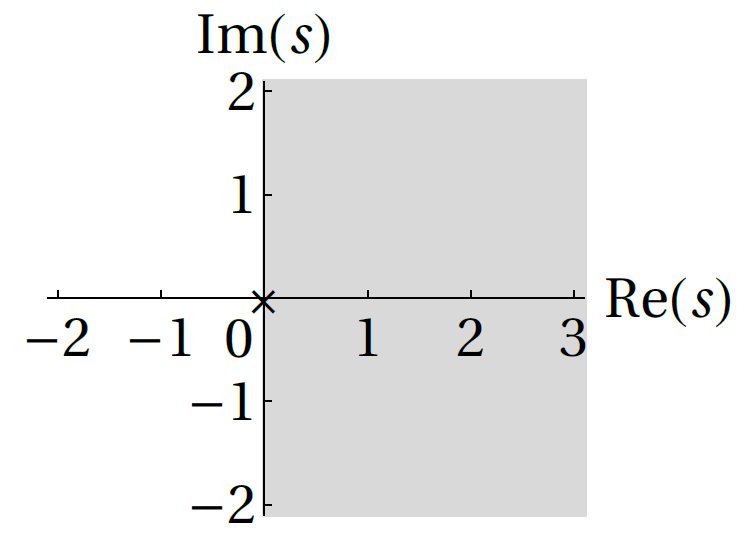
\includegraphics[width=\columnwidth]{images/konvergenzhalbebene.png} 
\end{minipage}
\hfill
\begin{minipage}[c]{0.48\columnwidth}
    Die Halbebene wird durch die \textbf{am weitesten rechts liegende Polstelle} von $F(s)$ begrenzt (Kreuzchen)
    \vspace{0.2cm}
    Falls $F(s)$ keine Polstelle hat, ist die Konvergenzhalbebene gleich $\mathbb{C}$
\end{minipage}


\subsection{Zusammenhang LT und FT}{145}

Bei kausalen, stabilen und fourier-transformierbaren Signalen $f(t)$ kann man durch das Ersetzen von $s = \sigma + \jimg \omega$ 
durch $\jimg \omega$ (und umgekehrt) zwischen der einseitigen Laplace-Transformation und der Fourier-Transformation wechseln.

\vspace{0.2cm}

Kennt man die einseitige Laplace-Transformation $F(s)$ des kausalen Signals $f(t)$, so kann man folgende Aussagen machen:

\vspace{0.1cm}

\begin{itemize}
    \setlength\itemsep{3pt}
    \item Liegt die $\jimg \omega$-Achse im Konvergenzbereich von $F(s)$, so kann $s$ 
        durch $\jimg \omega$ ausgetauscht werden, um $F(\jimg \omega)$ zu erhalten. 
    \item Liegt die $\jimg \omega$-Achse ausserhalb des Konvergenzbereichs von 
        $F(s)$, so konvergiert die Fourier-Transformation $F(\jimg \omega)$ nicht.
    \item Liegt die $\jimg \omega$-Achse auf dem Rand des Konvergenzbereichs von
        $F(s)$, so \textbf{können} die Fourier-Transformation $F(\jimg \omega)$ und die
        einseitige Laplace-Transformation $F(s)$ übereinstimmen, \textbf{müssen aber nicht}.
\end{itemize}
